%-------------------------------------------------------------------------------

% This file is part of Code_Saturne, a general-purpose CFD tool.
%
% Copyright (C) 1998-2020 EDF S.A.
%
% This program is free software; you can redistribute it and/or modify it under
% the terms of the GNU General Public License as published by the Free Software
% Foundation; either version 2 of the License, or (at your option) any later
% version.
%
% This program is distributed in the hope that it will be useful, but WITHOUT
% ANY WARRANTY; without even the implied warranty of MERCHANTABILITY or FITNESS
% FOR A PARTICULAR PURPOSE.  See the GNU General Public License for more
% details.
%
% You should have received a copy of the GNU General Public License along with
% this program; if not, write to the Free Software Foundation, Inc., 51 Franklin
% Street, Fifth Floor, Boston, MA 02110-1301, USA.

%-------------------------------------------------------------------------------

\programme{gradrc}\label{ap:gradrc}

\vspace{1cm}
%-------------------------------------------------------------------------------
\section*{Fonction}
%-------------------------------------------------------------------------------

Le but de ce sous-programme est de calculer, au centre des cellules, le gradient
d'une fonction scalaire, \'egalement connue au centre des cellules.
Pour obtenir la valeur du gradient, une m\'ethode it\'erative de
reconstruction pour les maillages non orthogonaux est mise en
\oe uvre~: elle fait appel \`a un d\'eveloppement limit\'e d'ordre 1 en espace
sur la variable, obtenu \`a partir de la
valeur de la fonction et de son gradient au centre de la cellule. Cette
m\'ethode,
choisie comme option par d\'efaut, correspond \`a \var{IMRGRA}\,=\,0 et est utilis\'ee pour le calcul
des gradients de toutes les grandeurs. Cette technique est plus robuste mais beaucoup plus lente que la m\'ethode
 par moindres carr\'es correspondant \`a \var{IMRGRA}\,=\,1.

%%%%%%%%%%%%%%%%%%%%%%%%%%%%%%%%%%
%%%%%%%%%%%%%%%%%%%%%%%%%%%%%%%%%%
\section*{Discr\'etisation}
%%%%%%%%%%%%%%%%%%%%%%%%%%%%%%%%%%
%%%%%%%%%%%%%%%%%%%%%%%%%%%%%%%%%%

\subsection*{\bf M\'ethode g\'en\'erale}
\begin{figure}[h]
\parbox{8cm}{%
\centerline{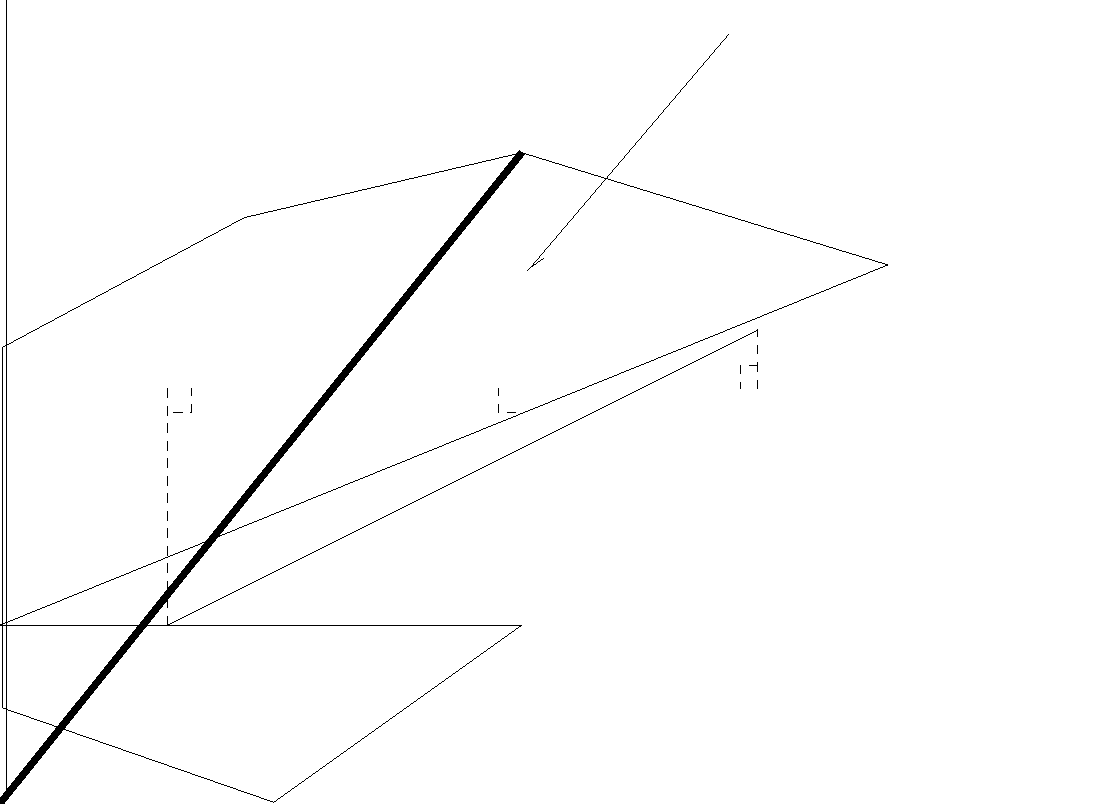
\includegraphics[height=4cm]{facette}}}
\parbox{8cm}{%
\centerline{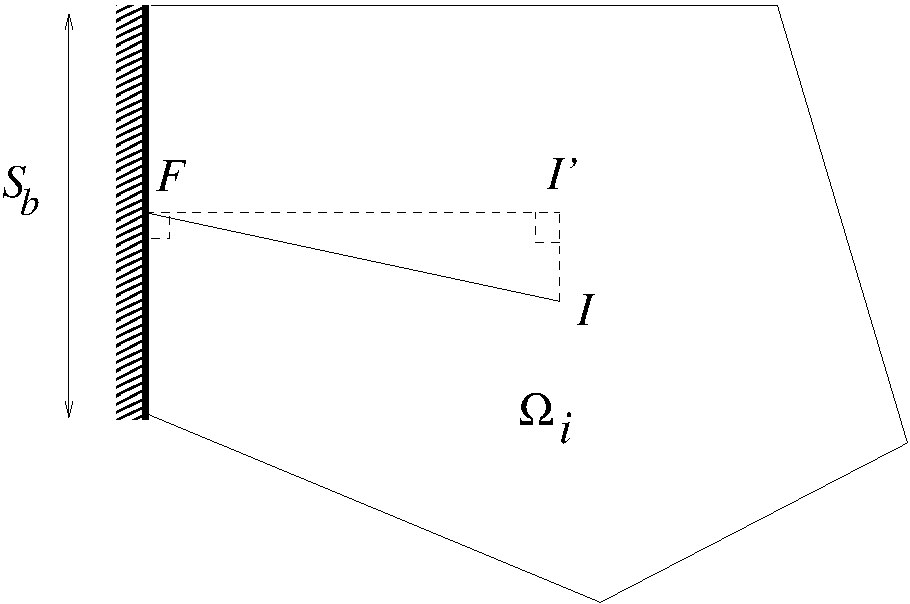
\includegraphics[height=4cm]{facebord}}}
\caption{\label{Base_Gradrc_fig_geom_gradmc}D\'efinition des diff\'erentes entit\'es
g\'eom\'etriques pour les faces internes (gauche) et de bord (droite).}
\end{figure}

On se reportera aux notations de la figure \ref{Base_Gradrc_fig_geom_gradmc}, qui
correspondent \`a celles employ\'ees dans le sous-programme \fort{gradmc}.
On cherche \`a calculer $\vect{G}_{\,c,i}$, gradient au centre de la cellule $i$ de la
fonction scalaire $P$. Le volume de la cellule $i$ est not\'e $\Omega_i$.
 Soit $\vect{G}_{\,f,ij}$ la valeur  du gradient \`a la face $ij$ dont les voisins sont les cellules $i$ et $j$.
%De m\^eme, on note $\vect{G}_{\,f,b_{\,ik}}$ la valeur du gradient \`a la face de
%bord $ik$ ($k^{\text{i\`eme}}$ face de bord appuy\'ee sur la cellule $i$).
$P_{ij}$ (resp. $P_{b,ik}$) repr\'esente la valeur estim\'ee de la variable $P$
\`a la face interne $ij$ (resp. \`a la face de bord $ik$, $k^{\text{i\`eme}}$
face de bord appuy\'ee sur la cellule $i$) de vecteur normal associ\'e
$\vect{S}_{ij}$ (resp. $\vect{S}_{b_{\,ik}}$).

Par  d\'efinition~:\\
\begin{equation}\notag
\begin{array}{ll}
\vect{G}_{\,c,i}&= (\grad {P})_{\,I} \\
\vect{G}_{\,f,ij}&= (\grad P)_{\,f,ij}\\
\end{array}
\end{equation}
On a~:
\begin{equation}\notag
\vect{G}_{\,f,ij}=(\grad {P})_{\,{O_{ij}}}= (\grad {P})_{\,{F_{ij}}}
  \text{   (\`a l'ordre 1 en $P$)}
\end{equation}
Afin de prendre en compte les non orthogonalit\'es \'eventuelles du maillage, on calcule le
gradient $\vect{G}_{\,c,i}$ en effectuant un d\'eveloppement limit\'e d'ordre
1 en espace. On obtient alors~:
\begin{equation}
\begin{array}{llll}
|\Omega_i|\,(\grad P)_{\,I}&\overset{\text{\it\small d\'ef}}{=}\displaystyle\int_{\Omega_i}{\grad{P}\, d\Omega}
=\sum\limits_{j\in Vois(i)}P_{\,ij}\,{\vect S_{\,ij}} + \sum\limits_{k\in {\gamma_b(i)}} P_{\,b_{ik}}\,\vect{S}_{\,{b}_{ik}} \\
 &= \sum\limits_{j\in Vois(i)}[P_{O_{ij}}+ \vect{O_{\,ij}F_{\,ij}}\,.\,(\grad
P)_{\,{O_{ij}}}] \,{\vect S_{\,ij}}+ \sum\limits_{k\in {\gamma_b(i)}} (\var {INC}\,A_{\,b,ik} + B_{\,b,ik}\,P_{I'} )\,\vect{S}_{\,{b}_{ik}}\\
 &= \sum\limits_{j\in Vois(i)}\left[\,(\alpha_{\,ij}\,P_I +
(1 - \alpha_{\,ij})\,P_J)\,\right]\,{\vect S_{\,ij}}
 +\sum\limits_{j\in Vois(i)}\left[\vect{O_{\,ij}F_{\,ij}}\,.\,(\grad
P)_{\,f,ij}\right]\,{\vect S_{\,ij}}\\
&+ \sum\limits_{k\in {\gamma_b(i)}} (\var{INC}\,A_{\,b,ik} + B_{\,b,ik}\,P_{I'})\,\vect{S}_{\,{b}_{ik}}\\
\end{array}
\end{equation}

La variable $\var{INC}$ permet d'affecter correctement les conditions aux limites des
quantit\'es dont on veut prendre le gradient. En effet,\\
$\bullet\ $ $\var{INC} = 1$ correspond \`a un calcul de gradient de variable totale et
donc \`a des conditions aux limites standards,\\
$\bullet\ $ $\var{INC} = 0$ correspond \`a un calcul de variable en incr\'ement et donc
\`a des conditions aux limites associ\'ees homog\`enes.\\

En faisant une approximation sur $P$ d'ordre 1 en espace \`a nouveau~:
\begin{equation}\notag
\left\{\begin{array}{ll}
(\grad P)_{\,f,ij}& = \displaystyle\frac{1}{2}\left[(\grad P)_{\,I} +(\grad P)_{\,J}\right]\\
P_{I'}&= P_I + \vect {II'}\,.\,(\grad P)_{\,I}\\
\end{array}\right .
\end{equation}

d'o\`u :

\begin{multline}\notag
|\Omega_i|\,\vect{G}_{\,c,i}= \sum\limits_{j\in Vois(i)}\left[(\alpha_{\,ij}\,P_I
+ (1 - \alpha_{\,ij})\,P_J)\, + \frac{1}{2}\,\vect{O_{\,ij}F_{\,ij}}\,.\,
\left(\,\vect{G}_{\,c,i} +\vect{G}_{\,c,j}\right)\right]\,{\vect S_{\,ij}}\\
+\sum\limits_{k\in {\gamma_b(i)}}\left[ \var{INC}\,A_{\,b,ik} +
B_{\,b,ik}\,P_{I} + B_{\,b,ik}\,\vect {II'}\,.\,\vect{G}_{\,c,i}
\right]\,\vect{S}_{\,{b}_{ik}}
\end{multline}
en notant $\displaystyle\alpha_{ij}=\frac{\overline{FJ'}}{\overline{I'J'}}$.

On regroupe \`a gauche les termes en $\vect{G}_{\,c,i}$ et on obtient~:
\begin{multline}\label{Base_Gradrc_eq_reconstruction}
|\Omega_i|\,\vect{G}_{\,c,i} -
\sum\limits_{j\in Vois(i)}\frac{1}{2}\,(\vect{O_{\,ij}F_{\,ij}}\,.\,\vect{G}_{\,c,i})\vect{S}_{\,ij}
-\sum\limits_{k\in {\gamma_b(i)}} B_{\,b,ik}\,(\vect{II'}\,.\,\vect{G}_{\,c,i})\,\vect{S}_{\,b_{ik}}
= \\
\sum\limits_{j\in Vois(i)}\left[
(\alpha_{\,ij}\,P_I + (1 - \alpha_{\,ij})\,P_J)\right]\,{\vect{S}_{\,ij}}
+\sum\limits_{j\in Vois(i)}\frac{1}{2}\,(\vect{O_{\,ij}F_{\,ij}}\,.\,\vect{G}_{\,c,j})\vect{S}_{\,ij}\\
+\sum\limits_{k\in {\gamma_b(i)}}(\var{INC}\,A_{\,b,ik} + B_{\,b,ik}\,P_{I})\,\vect{S}_{\,{b}_{ik}}
\end{multline}

ce qui donne pour la direction $\eta$ ($\eta ,\,\beta = \, x, \,y\,\, \text{ou} \, z$)  :
\begin{multline}\label{Base_Gradrc_eq_reconstruction_comp}
|\Omega_i|\,{G}_{\,c,i,\eta} -
\sum\limits_{j\in Vois(i)}\frac{1}{2}\,\left(\sum\limits_{\beta}(\vect{O_{\,ij}F_{\,ij}})_{,\,\beta}\,{G}_{\,c,i,\,\beta}\right){S}_{\,ij,\,\eta}
-\sum\limits_{k\in {\gamma_b(i)}} B_{\,b,ik}\,\left(\sum\limits_{\beta}(\vect{II'})_{,\,\beta}\,{G}_{\,c,i,\,\beta}\right)\,{S}_{\,b_{ik},\,\eta}
= \\
\sum\limits_{j\in Vois(i)}\left[
(\alpha_{\,ij}\,P_I + (1 - \alpha_{\,ij})\,P_J)\right]\,{{S}_{\,ij,\,\eta}}
+\sum\limits_{j\in Vois(i)}\frac{1}{2}\,\left(\sum\limits_{\beta}(\vect{O_{\,ij}F_{\,ij}})_{,\,\beta}\,{G}_{\,c,j,\,\beta}\right){S}_{\,ij,\,\eta}\\
+\sum\limits_{k\in {\gamma_b(i)}}(\var{INC}\,A_{\,b,ik} + B_{\,b,ik}\,P_{I})\,{S}_{\,{b}_{ik},\,\eta}
\end{multline}
\subsection*{\bf Cas sans reconstruction des non orthogonalit\'es}
Lorsque le maillage est orthogonal ou lorsqu'on ne veut pas reconstruire, seules
les contributions d'ordre $0$ au centre des cellules interviennent dans le
calcul du gradient ($\vect{II'} = \vect{0}$, $\vect{OF} = \vect{0}$)~:
\begin{equation}\notag
\begin{array}{ll}
|\Omega_i|\,\vect{G}_{\,c,i}&\overset{\text{\it\small d\'ef}}{=} \displaystyle\int_{\Omega_i}{\grad{P}\, d\Omega}
=\sum\limits_{j\in Vois(i)}P_{\,ij}\,{\vect S_{\,ij}} + \sum\limits_{k\in {\gamma_b(i)}} P_{\,b,ik}\,\vect{S}_{\,{b}_{ik}} \\
 &= \sum\limits_{j\in Vois(i)}\left[\,(\alpha_{\,ij}\,P_I +
(1 - \alpha_{\,ij})\,P_J)\,\right]\,{\vect S_{\,ij}}
+ \sum\limits_{k\in {\gamma_b(i)}} (\var{INC}\,A_{\,b,ik} + B_{\,b,ik}\,P_I )\,\vect{S}_{\,{b}_{ik}}\\
\end{array}
\end{equation}
d'o\`u :
\begin{multline}\label{Base_Gradrc_eq_nonreconstruction}
\vect{G}_{\,c,i}=\frac{1}{|\Omega_i|}\,.\left[\sum\limits_{j\in
Vois(i)}\left[\alpha_{\,ij}\,P_I + (1 - \alpha_{\,ij})\,P_J)\, \right]\,{\vect S_{\,ij}}\right.
+\left.\sum\limits_{k\in {\gamma_b(i)}}(\var{INC}\,A_{\,b,ik} + B_{\,b,ik}\,P_I
)\,\vect{S}_{\,{b}_{ik}} \right]
\end{multline}

\minititre{Remarque}
Le gradient non reconstruit $ \vect{G}_{\,c,i}^{NRec} $ se calcule donc tr\`es
facilement et directement {\it via} l'\'equation~(\ref{Base_Gradrc_eq_nonreconstruction}).
Il n'est cependant pas consistant sur maillage non orthogonal.

\subsection*{\bf Reconstruction}
\subsubsection*{\bf M\'ethode de r\'esolution}

Afin de pouvoir r\'esoudre le syst\`eme (\ref{Base_Gradrc_eq_reconstruction}), on va
impliciter les termes en $\vect{G}_{\,c,i}$, expliciter ceux en
$\vect{G}_{\,c,j}$ et raisonner de facon it\'erative en introduisant une suite
d'incr\'ements~$(\delta\,\vect{G}^{\,k}_{\,i})_{k\in \mathbb{N}}$ d\'efinie par~:\\
\begin{equation}
\left\{\begin{array}{l}
\delta\,\vect{G}^{\,0}_{\,i} = \vect{G}_{\,c,i}^{NRec}\\
\delta\,\vect{G}^{\,k+1}_{\,i} = \vect{G}^{k+1}_{\,c,i}-\vect{G}^k_{\,c,i}  \end{array}\right.
\end{equation}

et de syst\`eme associ\'e, dans la direction $\eta$~:

\begin{multline}\label{Base_Gradrc_eq_reconstruction_comp2}
|\Omega_i|\,{G}^{\,k+1}_{\,c,i,\eta} -
\sum\limits_{j\in Vois(i)}\frac{1}{2}\,\left(\sum\limits_{\beta}(\vect{O_{\,ij}F_{\,ij}})_{,\,\beta}\,{G}^{\,k+1}_{\,c,i,\,\beta}\right){S}_{\,ij,\,\eta}
-\sum\limits_{k\in {\gamma_b(i)}} B_{\,b,ik}\,\left(\sum\limits_{\beta}(\vect{II'})_{,\,\beta}\,{G}^{\,k+1}_{\,c,i,\,\beta}\right)\,{S}_{\,b_{ik},\,\eta}\\
= \sum\limits_{j\in Vois(i)}\left[
(\alpha_{\,ij}\,P_I + (1 - \alpha_{\,ij})\,P_J)\right]\,{{S}_{\,ij,\,\eta}}
+\sum\limits_{j\in Vois(i)}\frac{1}{2}\,\left(\sum\limits_{\beta}(\vect{O_{\,ij}F_{\,ij}})_{,\,\beta}\,{G}^{\,k}_{\,c,j,\,\beta}\right){S}_{\,ij,\,\eta}\\
+\sum\limits_{k\in {\gamma_b(i)}}(\var{INC}\,A_{\,b,ik} + B_{\,b,ik}\,P_{I})\,{S}_{\,{b}_{ik},\,\eta}
\end{multline}\\
ou, comme :
\begin{equation}\notag
 \vect{G}^{k+1}_{\,c,i}= \vect{G}^k_{\,c,i}+ \delta\,\vect{G}^{\,k+1}_{\,i}
\end{equation}

\begin{multline}\label{Base_Gradrc_eq_reconstruction_increment}
|\Omega_i|\,{\delta\,G}^{\,k+1}_{\,i,\,\eta} -
\sum\limits_{j\in Vois(i)}\frac{1}{2}\,\left(\sum\limits_{\beta}(\vect{O_{\,ij}F_{\,ij}})_{,\,\beta}\,{\delta\,G}^{\,k+1}_{\,c,i,\,\beta}\right){S}_{\,ij,\,\eta}
-\sum\limits_{k\in {\gamma_b(i)}} B_{\,b,ik}\,\left(\sum\limits_{\beta}(\vect{II'})_{,\,\beta}\,{\delta\,G}^{\,k+1}_{\,c,i,\,\beta}\right)\,{S}_{\,b_{ik},\,\eta}\\
= -|\Omega_i|\,{G}^{\,k}_{\,c,i,\eta}
 + \sum\limits_{j\in Vois(i)}\left[
(\alpha_{\,ij}\,P_I + (1 - \alpha_{\,ij})\,P_J)\right]\,{{S}_{\,ij,\,\eta}}\\
+ \sum\limits_{j\in Vois(i)}\left(\sum\limits_{\beta}(\vect{O_{\,ij}F_{\,ij}})_{,\,\beta}\,\,\frac{1}{2}\,({G}^{\,k}_{\,c,i,\,\beta}+\,{G}^{\,k}_{\,c,j,\,\beta})\right){S}_{\,ij,\,\eta}\\
+\sum\limits_{k\in {\gamma_b(i)}}(\var{INC}\,A_{\,b,ik} +
B_{\,b,ik}\,(P_{I} + \,\left(\sum\limits_{\beta}(\vect{II'})_{,\,\beta}\,{G}^{\,k}_{\,c,i,\,\beta}\right)))\,{S}_{\,{b}_{ik},\,\eta}
\end{multline}\\


L'\'equation (\ref{Base_Gradrc_eq_reconstruction_increment}) conduit \`a un syst\`eme matriciel local par rapport \`a chacune des trois composantes (${\delta\,G}^{\,k+1}_{\,i,x},{\delta\,G}^{\,k+1}_{\,i,y},{\delta\,G}^{\,k+1}_{\,i,z}$) du vecteur
inconnu $ \delta\,\vect{G}^{\,k+1}_{\,i}$. On obtient donc, pour chaque cellule~$i$, le syst\`eme $3\times3$ suivant~:
\begin{equation}\label{Base_Gradrc_eq_systeme_matriciel_gradrc}
\underbrace{
\left[\begin{array}{ccc}
\displaystyle
C_{i,x\,x}
& C_{i,x\,y}
& C_{i,x\,z}\\
\displaystyle
C_{i,y\,x}
& C_{i,y\,y}
& C_{i,y\,z}\\
\displaystyle
C_{i,z\,x}
& C_{i,z\,y}
& C_{i,z\,z}
\end{array}\right]
}_{\tens{C}_{\,i}}
\underbrace{
\left[\begin{array}{c}
{\delta\,G}^{\,k+1}_{\,i,x}\\{\delta\,G}^{\,k+1}_{\,i,y}  \\ {\delta\,G}^{\,k+1}_{\,i,z}
\end{array}\right]
}_{\delta\,\vect{G}^{\,k+1}_{\,i}}
=
\underbrace{
\left[\begin{array}{c}
\displaystyle
R^{\,k+1}_{i,x}\\
\displaystyle
R^{\,k+1}_{i,y}\\
\displaystyle
R^{\,k+1}_{i,z}
\end{array}\right]
}_{\vect{R}^{\,k+1}_{i}}
\end{equation}

avec, ($\eta ,\,\beta = \, x, \,y\,\, \text{ou} \, z$) :

\begin{equation}\label{Base_Gradrc_eq_second_membre}
\left\{\begin{array}{lll}
C_{i,\eta\,\eta} &= |\Omega _i| - \displaystyle \frac{1}{2}\sum\limits_{j\in
Vois(i)}(\vect{O_{\,ij}F_{\,ij}})_{,\,\eta}\,S_{\,ij,\,\eta} -\sum\limits_{k\in
\gamma_b(i)} B_{\,b,ik}\,(\vect{II'})_{,\,\eta}\,S_{\,{b}_{ik},\,\eta}\\
C_{i,\eta\,\beta} &= - \displaystyle \frac{1}{2}\sum\limits_{j\in
Vois(i)}(\vect{O_{\,ij}F_{\,ij}})_{,\,\beta}\,S_{\,{ij},\,\eta}
 -\sum\limits_{k\in \gamma_b(i)}
B_{\,b,ik}\,(\vect{II'})_{,\,\beta}\,S_{\,{b}_{ik},\,\eta}  &\text{ pour $\eta
\ne \beta$}\\
R^{\,k+1}_{i,\eta} &=  -|\Omega_i|\,{G}^{\,k}_{\,c,i,\eta}
 + \sum\limits_{j\in Vois(i)}\left[
(\alpha_{\,ij}\,P_I + (1 - \alpha_{\,ij})\,P_J)\right]\,{{S}_{\,ij,\,\eta}}\\
&+ \sum\limits_{j\in Vois(i)}\left(\sum\limits_{\beta}(\vect{O_{\,ij}F_{\,ij}})_{,\,\beta}\,\,\displaystyle\frac{1}{2}\,({G}^{\,k}_{\,c,i,\,\beta}+\,{G}^{\,k}_{\,c,j,\,\beta})\right){S}_{\,ij,\,\eta}\\
&+\displaystyle{\sum\limits_{k\in {\gamma_b(i)}}(\var{INC}\,A_{\,b,ik} +
B_{\,b,ik}\,\left(P_{I} + \,\left(\sum\limits_{\beta}(\vect{II'})_{,\,\beta}\,{G}^{\,k}_{\,c,i,\,\beta}\right)\right))\,{S}_{\,{b}_{ik},\,\eta}}
\end{array}\right.
\end{equation}

L'inversion de la matrice $\tens{C}_{\,i}$ permet de calculer
$(\delta\,\vect{G}^{\,k+1}_{\,i})$ et donc $(\vect{G}^{\,k+1}_{\,i})$. Les
it\'erations s'arr\^etent lorsque la norme euclidienne du second membre
$\vect{R}^{\,k+1}_{\,i}$ tend vers z\'ero ({\it i.e.} lorsque la norme
euclidienne  de
$(\delta\,\vect{G}^{\,k}_{\,i})$ tend vers z\'ero) ou lorsque le nombre
d'it\'erations en $k$ fix\'e maximal est atteint.

\minititre{Remarque 3}
Pour les conditions aux limites en pression, un traitement particulier est mis
en  \oe uvre, surtout utile dans les cas o\`u un gradient de pression (hydrostatique
ou autre) n\'ecessite une attention sp\'ecifique aux bords, o\`u une condition
\`a la limite de type Neumann homog\`ene est g\'en\'eralement inadapt\'ee. Soit
$P_{F_{\,b_{\,ik}}}$ la  valeur de la pression \`a la face associ\'ee, que
l'on veut calculer.

On note que ~:
\begin{equation}\notag
\vect{I'F}_{\,b_{\,ik}} \,.\,(\grad P)_I = \vect{I'F}_{\,b_{\,ik}}
\,.\,\vect{G}_{\,c,i} = \overline{I'F}_{\,b_{\,ik}} \,.\left. \displaystyle\frac{\delta P}{\delta
n}\right|_{F_{\,b_{\,ik}}}
\end{equation}
avec les conventions pr\'ec\'edentes.\\
\paragraph{\bf Sur maillage orthogonal }
On se place dans le cas d'un maillage orthogonal , {\it i.e.} pour
toute cellule $\Omega_I$, $I$ et son projet\'e $I'$ sont identiques.
Soit $M_{\,b_{\,ik}}$ le milieu du segment $IF_{\,b_{\,ik}}$.\\
On peut \'ecrire les \'egalit\'es suivantes~:
\begin{equation}\notag
\begin{array}{ll}
P_{F_{\,b_{\,ik}}} & = P_{M_{\,b_{\,ik}}} + \overline{M_{\,b_{\,ik}}F_{\,b_{\,ik}}}\,.\left. \displaystyle\frac{\delta P}{\delta
n}\right|_{M_{\,b_{\,ik}}} +
\overline{M_{\,b_{\,ik}}F_{\,b_{\,ik}}}^{\,2}\,.\left.\displaystyle\frac{1}{2}\frac{{\delta}^{2} P}{\delta
n^2}\right|_{M_{\,b_{\,ik}}} + \mathcal{O}(h^3)\\
P_I & = P_{M_{\,b_{\,ik}}} + \overline{M_{\,b_{\,ik}}I}\,.
\left. \displaystyle\frac{\delta P}{\delta n}\right|_{M_{\,b_{\,ik}}} +
\overline{M_{\,b_{\,ik}}I}^{\,2}\,.\left.\displaystyle\frac{1}{2}
\frac{{\delta}^{2} P}{\delta n^2}\right|_{M_{\,b_{\,ik}}} + \mathcal{O}(h^3)
\end{array}
\end{equation}
avec $\overline{M_{\,b_{\,ik}}I} = - \overline{M_{\,b_{\,ik}}F_{\,b_{\,ik}}}$.\\
On obtient donc~:
\begin{equation}\label{Base_Gradrc_eq_orthogonal}
P_{F_{\,b_{\,ik}}} - P_I = \overline{IF}_{\,b_{\,ik}}\,.\left. \displaystyle\frac{\delta P}{\delta
n}\right|_{M_{\,b_{\,ik}}} + \mathcal{O}(h^3)
\end{equation}
Gr\^ace \`a la formule des accroissements finis :
\begin{equation}\label{Base_Gradrc_eq_derivee_normale}
\left. \displaystyle\frac{\delta P}{\delta n}\right|_{M_{\,b_{\,ik}}} =
\displaystyle\frac{1}{2}\left[\left. \displaystyle\frac{\delta P}{\delta
n}\right|_{I} +  \left. \displaystyle\frac{\delta P}{\delta
n}\right|_{F_{\,b_{\,ik}}}\right] + \mathcal{O}(h^2)
\end{equation}\\
On s'int\'eresse aux cas suivants :\\\\
\hspace*{0.5cm}{ $\bullet${\underline { condition \`a la limite de type Dirichlet}}}\\
$P_{F_{\,b_{\,ik}}} = P_{IMPOSE}$, aucun traitement particulier\\\\
\hspace*{0.5cm}{ $\bullet ${\underline { condition \`a la limite de type Neumann
homog\`ene standard}}}\\
On veut imposer :
\begin{equation}
\left. \displaystyle\frac{\delta P}{\delta n}\right|_{F_{\,b_{\,ik}}} = 0 + \mathcal{O}(h)
\end{equation}
On a~:
\begin{equation}\notag
\left. \displaystyle\frac{\delta P}{\delta n}\right|_{I} =
\displaystyle\left. \displaystyle\frac{\delta P}{\delta
n}\right|_{F_{\,b_{\,ik}}} + \mathcal{O}(h)
\end{equation}
et comme :
\begin{equation}
P_{F_{\,b_{\,ik}}} = P_I + \overline{IF}_{\,b_{\,ik}}\,.\left. \displaystyle\frac{\delta P}{\delta
n}\right|_I + \mathcal{O}(h^2)
\end{equation}
on en d\'eduit :
\begin{equation}
P_{F_{\,b_{\,ik}}} = P_I + \overline{IF}_{\,b_{\,ik}}\,.\left. \displaystyle\frac{\delta P}{\delta
n}\right|_{F_{\,b_{\,ik}}} + \mathcal{O}(h^2)
\end{equation}
soit~:
\begin{equation}
P_{F_{\,b_{\,ik}}} = P_I +  \mathcal{O}(h^2)
\end{equation}
On obtient donc une approximation d'ordre 1.\\
\hspace*{0.5cm}{ $\bullet ${\underline { condition \`a la limite de type Neumann homog\`ene am\'elior\'ee}}}\\
Des \'egalit\'es (\ref{Base_Gradrc_eq_orthogonal}, \ref{Base_Gradrc_eq_derivee_normale}), on tire~:
\begin{equation}\notag
P_{F_{\,b_{\,ik}}} = P_I +
\displaystyle\frac{1}{2}\,\overline{IF}_{\,b_{\,ik}}\,.\,\left. \displaystyle\frac{\delta P}{\delta
n}\right|_{I} + \mathcal{O}(h^3)
\end{equation}
On obtient donc une approximation d'ordre 2.\\
\hspace*{0.5cm}{$\bullet $ {\underline { condition \`a la limite de type
extrapolation du gradient}}$\ \ \left. \displaystyle\frac{\delta P}{\delta
n}\right|_{F_{\,b_{\,ik}}} = \displaystyle\left. \displaystyle\frac{\delta
P}{\delta n}\right|_{I}$}\\
Des deux \'egalit\'es (\ref{Base_Gradrc_eq_orthogonal}, \ref{Base_Gradrc_eq_derivee_normale}), on d\'eduit~:
\begin{equation}
P_{F_{\,b_{\,ik}}}= P_I + \overline{IF}_{\,b_{\,ik}}\,.\left. \displaystyle\frac{\delta P}{\delta
n}\right|_{I} + \mathcal{O}(h^3)
\end{equation}
On obtient donc \'egalement une approximation d'ordre 2.\\
\paragraph{\bf Sur maillage non orthogonal}
Dans ce cas, on peut seulement \'ecrire~:\\
\begin{equation}
P_{F_{\,b_{\,ik}}}  = P_{I'} +
\displaystyle\frac{1}{2}\,\vect{I'F}_{\,b_{\,ik}}\,.\,[\,(\grad P)_{I'} + (\grad
P)_{F_{\,b_{\,ik}}}\,] + \mathcal{O}(h^3)
\end{equation}
\hspace*{0.5cm}{ $\bullet ${\underline { condition \`a la limite de type Dirichlet}}\\
$P_{F_{\,b_{\,ik}}} = P_{IMPOSE}$, toujours aucun traitement particulier\\\\
\hspace*{0.5cm}{ $\bullet ${\underline { condition \`a la limite de type Neumann
homog\`ene standard}}}\\
On veut :
\begin{equation}
\left. \displaystyle\frac{\delta P}{\delta n}\right|_{F_{\,b_{\,ik}}} = 0 + \mathcal{O}(h)
\end{equation}
ce qui entra\^\i ne :
\begin{equation}\label{Base_Gradrc_eq_ortho}
\vect{I'F}_{\,b_{\,ik}} \,.\,(\grad P)_{F_{\,b_{\,ik}}} = \mathcal{O}(h^2)
\end{equation}
On peut \'ecrire :
\begin{equation}\notag
(\grad P)_{I'} = (\grad P)_{F_{\,b_{\,ik}}} +  \mathcal{O}(h)
\end{equation}
d'o\`u~:
\begin{equation}
P_{F_{\,b_{\,ik}}} = P_{I'}  + \mathcal{O}(h^2)
\end{equation}
On obtient donc une approximation d'ordre 1.\\

\hspace*{0.5cm}{$\bullet $ {\underline { condition \`a la limite de type Neumann homog\`ene am\'elior\'ee}}}\\
Le gradient n'est connu qu'au centre des cellules $I$ et non aux points $I'$.
\begin{equation}\notag
(\grad P)_{I'} = (\grad P)_I +  \mathcal{O}(h)
\end{equation}
d'o\`u :
\begin{equation}
\begin{array}{ll}
P_{F_{\,b_{\,ik}}} & = P_{I'} + \displaystyle\frac{1}{2}\,\vect{I'F}_{\,b_{\,ik}}\,.\,[\,(\grad P)_{I'} +
(\grad P)_{F_{\,b_{\,ik}}}\,] + \mathcal{O}(h^3)\\
& = P_{I'} + \displaystyle\frac{1}{2}\,\vect{I'F}_{\,b_{\,ik}}\,.\,[\,(\grad P)_{I} +
(\grad P)_{F_{\,b_{\,ik}}}\,] + \mathcal{O}(h^2)\
\end{array}
\end{equation}
Compte-tenu de la condition impos\'ee et de l'\'equation ($\ref{Base_Gradrc_eq_ortho}$), seule la contribution en $I$ reste.
\begin{equation}
\begin{array}{ll}
P_{F_{\,b_{\,ik}}}  = P_{I'} + \displaystyle\frac{1}{2}\,\vect{I'F}_{\,b_{\,ik}}\,.\,(\grad P)_{I}
 + \mathcal{O}(h^2)\\
\end{array}
\end{equation}
On obtient donc une approximation d'ordre 1.\\
\hspace*{0.5cm}{ $\bullet $ {\underline { condition \`a la limite de type extrapolation du gradient}} $\ \ \left. \displaystyle\frac{\delta P}{\delta n}\right|_{F_{\,b_{\,ik}}} =
\displaystyle\left. \displaystyle\frac{\delta P}{\delta n}\right|_{I}$}\\
En tenant compte de cette \'egalit\'e, l'expression de $P_{F_{\,b_{\,ik}}}$ devient :
\begin{equation}
P_{F_{\,b_{\,ik}}}  = P_{I'} + \displaystyle\,\vect{I'F}_{\,b_{\,ik}}\,.\,(\grad P)_{I}
 + \mathcal{O}(h^2)
\end{equation}
On obtient \'egalement une approximation d'ordre 1.\\

\hspace*{0.5cm}{\bf $\bullet $ Conclusion }\\
On peut r\'ecapituler toutes ces situations {\it via} la formule :
\begin{equation}\notag
P_{F_{\,b_{\,ik}}}\,=\,P_{I'}+ \,\var{EXTRAP}\,\,(\vect{I'F}_{\,b_{\,ik}}\,.\,(\grad P)_{I})
\end{equation}
avec $\var{EXTRAP}$ valant $0$, $0.5$ ou $1$.\\

Il ne faut en aucun cas utiliser $\var{EXTRAP}$ avec des conditions de type
Neumann non homog\`enes $\left. \displaystyle\frac{\delta P}{\delta
n}\right|_{F}$ = $g_{\,bord}$ , $g_{\,bord}$ donn\'ee non nulle ou de type
Robin (mixtes) plus g\'en\'eralement \\ $a P_{F_{\,b_{\,ik}}} + b \left. \displaystyle\frac{\delta
P}{\delta n}\right|_{F_{\,b_{\,ik}}} = g_{\,bord}$, le recours \`a  $
\var{EXTRAP}$ n'ayant plus aucun sens.

%%%%%%%%%%%%%%%%%%%%%%%%%%%%%%%%%%
%%%%%%%%%%%%%%%%%%%%%%%%%%%%%%%%%%
\section*{Mise en \oe uvre}
%%%%%%%%%%%%%%%%%%%%%%%%%%%%%%%%%%
%%%%%%%%%%%%%%%%%%%%%%%%%%%%%%%%%%


La variable dont il faut calculer le gradient est contenue dans le tableau
\var{PVAR}. Les conditions aux limites associ\'ees sont disponibles au travers
des tableaux \var{COEFAP} et \var{COEFBP} qui repr\'esentent respectivement les
grandeurs $A$ et $B$ utilis\'ees ci-dessus. Les trois composantes du gradient
sont contenues, en sortie du sous-programme, dans les tableaux \var{DPDX},
\var{DPDY} et \var{DPDZ}.\\

\etape{Initialisations}
Le tableau (\var{BX}, \var{BY}, \var{BZ}) du second membre $\vect{R}_{\,i}$ est initialis\'e \`a
z\'ero.\\
Le calcul du gradient cellule non reconstruit $\vect{G}^{NRec}_{\,c,i}$ est
r\'ealis\'e et stock\'e dans les tableaux \var{DPDX}, \var{DPDY} et \var{DPDZ}. Si
aucune reconstruction n'est \`a faire, on a fini.\\
\hspace*{1cm}\subsection*{\bf  Reconstruction}
Sinon, on cherche \`a r\'esoudre le syst\`eme (\ref{Base_Gradrc_eq_reconstruction_increment}) en incr\'ements de
gradient ${\delta\,\vect{G}}^{\,k+1}_{\,i}$. Le gradient non reconstruit
constitue alors une premi\`ere estimation du gradient \`a calculer par
incr\'ements.\\
On effectue les op\'erations suivantes~:
\hspace*{1cm}\subsubsection*{\bf Phase pr\'eliminaire}
\hspace*{1,5cm}{\bf Calcul de la matrice, hors boucle en $k$}\\
Les \var{NCEL} matrices $\tens{C}_{\,i}$ (matrices non sym\'etriques $3\times 3$) sont
stock\'ees dans le tableau \var{COCG},
(de dimension $\text{\var{NCELET}}\times 3\times 3$). Ce dernier est initialis\'e \`a z\'ero,
puis son remplissage est r\'ealis\'e dans des boucles sur les faces internes et
les faces de bord. Pour \'eviter de r\'ealiser plusieurs fois les m\^emes
calculs g\'eom\'etriques, on conserve, en sortie de sous-programme, dans le
tableau \var{COCG}, l'inverse des \var{NCEL} matrices $\tens{C}_{\,i}$.


\hspace*{2cm}{\bf Cellule ne poss\'edant pas de face de bord }\\
Lorsque, pour une cellule, aucune des faces n'est une face de bord du domaine,
l'expression de la matrice $\tens{C}_{\,i}$ ne fait intervenir que des grandeurs
g\'eom\'etriques. Son inverse peut \^etre donc calcul\'e une seule fois, stock\'e dans
\var{COCG} et r\'eutilis\'e si l'on rappelle \fort{gradrc} s\'equentiellement et
si on est sur un maillage fixe (indicateur \var{ICCOCG} positionn\'e \`a 0).

\hspace*{2cm}{\bf Cellule poss\'edant au moins une face de bord }\\
Lorsque l'ensemble des faces d'une cellule contient au moins une face de bord
du domaine, un terme contributeur aux matrices  $\tens{C}_{\,i}$ est
sp\'ecifique \`a la variable dont on cherche
\`a calculer le gradient, au travers du coefficient $B_{\,b,ik}$
issu des conditions aux limites. Il s'agit de~:

\begin{equation}\notag
- \displaystyle\sum\limits_{k\in\gamma_b(i)}
B_{\,b,ik}\,(\vect{II'})_{\,\beta} \,S_{\,{b}_{ik},\,\eta}
\end{equation}

Si, lors de l'appel pr\'ec\'edent\footnote{donc, \`a partir du second appel au
moins}  \`a \fort{gradrc},
les conditions aux limites relatives \`a la
variable $P$ trait\'ee conduisaient \`a des valeurs identiques de $B_{\,b,ik}$, les
matrices $\tens{C}_{\,i}$ sont donc inchang\'ees et l'inverse  est encore
disponible  dans \var{COCG}. Pour \'eviter de refaire les calculs associ\'es,
l'indicateur \var{ICCOCG}, pass\'e en argument, est alors positionn\'e \`a 0.

Si, au contraire, les valeurs de $B_{\,b,ik}$  sont diff\'erentes de celles de
l'appel pr\'ec\'edent, il est alors
indispensable de recalculer le terme et l'indicateur \var{ICCOCG} doit \^etre
positionn\'e \`a 1.\\\\
Toutefois compte-tenu du co\^ut total de l'inversion de ces matrices relativement
au co\^ut global du sous-programme, cette d\'emarche de stockage et donc
d'\'economie de temps C.P.U. est un peu
superflue et risque d'engendrer des erreurs (indicateur \var{ICCOCG}
positionn\'e \`a 0 au lieu de 1) beaucoup plus p\'enalisantes que l'\'eventuel
gain escompt\'e.\\\\
\hspace*{1,5cm}{\bf Inversion de la matrice}\\
%\hspace*{1,5cm}\etape{Inversion de la matrice}
On calcule les coefficients de la comatrice, puis l'inverse.
Pour des questions de vectorisation, la boucle sur les \var{NCEL} \'el\'ements
est remplac\'ee par une
s\'erie de boucles en vectorisation forc\'ee sur des blocs de \var{NBLOC=1024}
\'el\'ements. Le reliquat ($\var{NCEL}-E(\var{NCEL}/1024)\times 1024$) est
trait\'e apr\`es les boucles.
La matrice inverse est ensuite stock\'ee dans \var{COCG}.\\
\hspace*{1cm}\subsubsection*{\bf Phase it\'erative $k$, $k\in \mathbb{N}$}
On suppose  $\delta\,\vect{G}^{\,k}_{\,i}$ connu et donc  $\vect{G}^{k}_{\,c,i}$ pour $k$ donn\'e et sur
toute cellule $\Omega_{i}$ et on veut calculer
$\delta\,\vect{G}^{\,k+1}_{\,i}$ et $\vect{G}^{k+1}_{\,c,i}$ .\\

\hspace*{1,5cm}{\bf Calcul du second membre ${\vect{R}^{\,k+1}_{\,i}}$ et
r\'esolution}\\
Le calcul proprement dit du second membre ${\vect{R}^{\,k+1}_{\,i}} $
correspondant au syst\`eme (\ref{Base_Gradrc_eq_second_membre}) est effectu\'e et stock\'e
dans le tableau (\var{BX}, \var{BY}, \var{BZ}). Il est initialis\'e, \`a chaque
pas $k$, par la
valeur du gradient $\vect{G}^{k}_{\,c,i}$ multipli\'e par le
volume de la cellule $|\Omega_i|$, avec $\vect{G}^{0}_{\,c,i} = \vect{G}^{Nrec}_{\,c,i}$ . L'incr\'ement $(\delta\,\vect{G}^{\,k+1}_{\,i})$
de gradient est obtenu par $ {\tens{C}_{\,i}}^{-1}{\vect{R}^{\,k+1}_{\,i}}$ et
ajout\'e dans les tableaux \var{DPDX},
\var{DPDY} et \var{DPDZ} pour obtenir $\vect{G}^{k+1}_{\,c,i}$.\\

En ce qui concerne les conditions aux limites en pression, elles sont
trait\'ees comme suit dans \CS :
\begin{equation}\notag
\left\{\begin{array}{llll}
P_{I'}&=P_{I}+\vect{II'}.\vect{G}_{c,i}\\
P_{b,ik}& =\var{INC}\,A_{\,b,ik} + B_{\,b,ik}\,P_{I'} = \var{INC}\,A_{\,b,ik} + B_{\,b,ik}(P_{I}+\vect{II'}.\,\vect{G}_{\,c,i}) \\
P_{b_{1},ik}&= P_{I}+\vect{I{F_{\,ij}}}.\,\vect{G}_{\,c,i}\\
P_{f,\,b_{\,ik}}&= B_{\,b,ik}(\var{EXTRAP}\,P_{b_{1},ik} + (1 -\var{EXTRAP})\,P_{b,ik}) + (1 -
B_{\,b,ik})P_{b,ik}
\end{array}\right.
\end{equation}
ce qui correspond \`a :\\\\
\hspace*{1cm}{\tiny$\blacksquare$}\, lorsqu'on veut imposer des conditions de Dirichlet ($A_{\,b,ik} =
P_{F_{\,b_{\,ik}}}$, $B_{\,b,ik} = 0$),
\begin{equation}
P_{F_{\,b_{\,ik}}}  = P_{IMPOSE}
\end{equation}
pour toute valeur de \var{EXTRAP}.\\\\
\hspace*{1cm}{\tiny$\blacksquare$}\, lorsqu'on veut imposer des conditions de
flux ($A_{\,b,ik} = 0$, $B_{\,b,ik} = 1$) (condition de type Neumann)
\begin{equation}
P_{F_{\,b_{\,ik}}}  = \,\var{EXTRAP}\,\ (P_{I} + (\vect{IF}_{\,b_{\,ik}}\,.\,(\grad P)_{I})  + (1 -\,\var{EXTRAP}) P_{I'}
\end{equation}
seules trois valeurs de \var{EXTRAP} sont licites.\\\\
\hspace*{2cm}$\bullet $ avec un maillage non orthogonal \\\\
L'ordre obtenu est \'egal \`a 1 dans tous les cas.
\begin{equation}\notag
\begin{array}{llll}
\var{EXTRAP}&= 0 &\text{Neumann homog\`ene}&\ \  P_{F_{\,b_{\,ik}}} = P_{I'} + \mathcal{O}(h^2)\\
\var{EXTRAP}&= \displaystyle\frac{1}{2} &\text{Neumann homog\`ene am\'elior\'e}&\ \
P_{F_{\,b_{\,ik}}} = P_{I'} + \displaystyle\frac{1}{2}\,\vect{I'F}_{\,b_{\,ik}}\,.\,(\grad P)_{I}
+ \mathcal{O}(h^2)\\
\var{EXTRAP} &= 1&\text{extrapolation du gradient}&\ \
P_{F_{\,b_{\,ik}}} = P_{I'} + \vect{I'F}_{\,b_{\,ik}}\,.\,(\grad P)_{I} + \mathcal{O}(h^2)\\
\end{array}
\end{equation}\\\\
\hspace*{2cm}$\bullet $ avec un maillage orthogonal \\\\
On peut atteindre l'ordre deux.\\
\begin{equation}\notag
\begin{array}{lllll}
\var{EXTRAP} &= 0 &\text{Neumann homog\`ene}&
P_{F_{\,b_{\,ik}}}  = P_{I'} + \mathcal{O}(h^2)\\
&\ &\text{on est \`a l'ordre 1}\\
\var{EXTRAP} &=  \displaystyle\frac{1}{2} &\text{Neumann homog\`ene am\'elior\'e}&\ \
P_{F_{\,b_{\,ik}}}  = P_{I} + \displaystyle\frac{1}{2}\,\vect{IF}_{\,b_{\,ik}}\,.\,(\grad P)_{I}
+ \mathcal{O}(h^3)\\
&\ &\text{on est \`a l'ordre 2}\\
\var{EXTRAP} &= 1 &\text{extrapolation du gradient}&\ \
P_{F_{\,b_{\,ik}}}  = P_{I} + \vect{IF}_{\,b_{\,ik}}\,.\,(\grad P)_{I} +
\mathcal{O}(h^3)\\
&\ &\text{on est \`a l'ordre 2}\\
\end{array}
\end{equation}

\hspace*{1,5cm}{\bf Test de convergence de la m\'ethode it\'erative de r\'esolution}\\
On calcule la norme euclidienne $\var {RESIDU}$ du second membre (\var{BX},
\var{BY}, \var{BZ}).\\
On arr\^ete les it\'erations sur $k$ si le test de
convergence pour cette norme ou le nombre de
sweeps maximal \var{NSWRGP} est atteint. La valeur par d\'efaut de \var{NSWRGP}  est fix\'ee \`a 100, ce
qui permet un calcul suffisamment pr\'ecis pour l'ordre d'espace
consid\'er\'e.\\
Sinon, on continue d'it\'erer sur $k$.
%%%%%%%%%%%%%%%%%%%%%%%%%%%%%%%%%%
%%%%%%%%%%%%%%%%%%%%%%%%%%%%%%%%%%
\section*{Points \`a traiter}
%%%%%%%%%%%%%%%%%%%%%%%%%%%%%%%%%%
%%%%%%%%%%%%%%%%%%%%%%%%%%%%%%%%%%
\etape{Vectorisation forc\'ee}
Il est peut-\^etre possible de s'affranchir du d\'ecoupage en boucles de 1024 si
les compilateurs sont capables
d'effectuer la vectorisation sans cette aide. On note cependant que ce
d\'ecoupage en boucles de 1024 n'a pas de co\^ut CPU suppl\'ementaire, et que
le co\^ut m\'emoire associ\'e est n\'egligeable.
Le seul inconv\'enient r\'eside dans la relative complexit\'e  de l'\'ecriture.

\etape{Traitement des conditions aux limites de pression}
Actuellement, l'ordre deux d\'ecrit dans le cas $\var{EXTRAP} = \displaystyle \frac{1}{2}$ relativement
aux conditions aux limites de pression n'existe pas dans \CS \ en non
orthogonal. Mais en a-t-on vraiment besoin ?

\etape{M\'ethode it\'erative de r\'esolution}
La m\'ethode it\'erative de r\'esolution adopt\'ee dans ce sous-programme  marche, {\it
i.e.} converge, mais ne rentre dans aucun cadre th\'eorique pr\'ecis. Des
r\'eflexions sur le sujet pourraient \'eventuellement permettre d'exhiber certaines propri\'et\'es
des matrices consid\'er\'ees, cerner les limites d'application ou expliquer
certains comportements.
